\documentclass[xcolor=dvipsnames]{beamer}
\usepackage[czech]{babel}
\usepackage[utf8]{inputenc}
\usepackage{graphics}
\usepackage{color}
\usepackage{amsfonts}
\usepackage{wrapfig}
\usepackage[export]{adjustbox}

\newcommand{\myuv}[1]{\quotedblbase #1\textquotedblleft}

\useinnertheme{rectangles}
\definecolor{Mycolor}{HTML}{536887}
\setbeamercolor{title}{fg=White,bg=Mycolor}
\setbeamercolor{frametitle}{fg=White,bg=Mycolor}

\begin{document}
%~^~%~^~%~^~%~%~^~%~%~^~%~% TITLE PAGE ~^~%~%~^~%~%~^~%~%~^~%~%~^~%
	
	\title{\textsc{\huge{Typografia}}}
	\subtitle{\textsc{\small{História a~stručná charakteristika}}}
	\author{\scriptsize{Martina Grzybowská\\xgrzyb00@stud.fit.vutbr.cz}}
	\date{\scriptsize{5. máj 2016}}
	\maketitle

%~^~%~^~%~^~%~%~^~%~%~^~%~%~^~%~%~^~%~%~^~%~%~^~%~%~^~%~%~^~%~%~^~%

\begin{frame}{\textsc{\large{Čo to je typografia?}}}
	\begin{center}
		Typografia je forma jazyka. Je tým, čo dáva textu vizuálnu podobu.
	\end{center}
	\begin{figure}[ht]
		\begin{center}
			\scalebox{0.3}{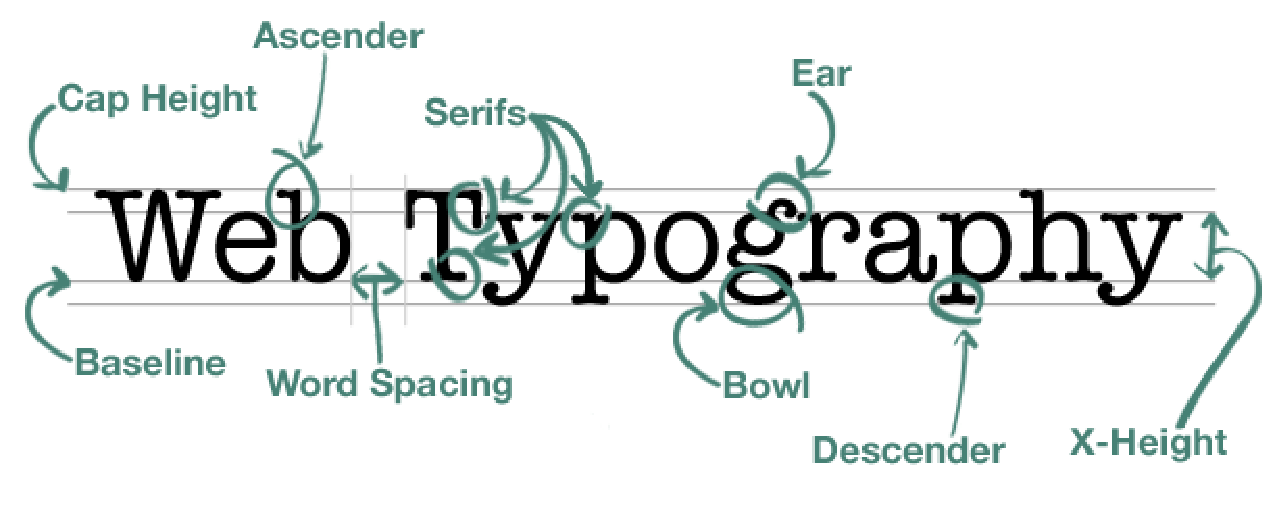
\includegraphics{typo.eps}}
    		\caption{\textit{Ukážka typografie}}
		\end{center}
	\end{figure}
\end{frame}

%~^~%~^~%~^~%~%~^~%~%~^~%~%~^~%~%~^~%~%~^~%~%~^~%~%~^~%~%~^~%~%~^~%

\begin{frame}{\textsc{\large{Čo to je typografia?}}}
	\begin{center}
		\textbf{\color{red}Vhodným} výberom písma môžeme u čitateľa vzbudiť emócie alebo zapôsobit na istú cieľovú skupinu. 
	\end{center}
	\begin{figure}[ht]
		\begin{center}
			\scalebox{0.5}{
\includegraphics{funeral.eps}}
    		\caption{\textit{Ukážka nevhodného výberu písma}}
		\end{center}
	\end{figure}
\end{frame}

%~^~%~^~%~^~%~%~^~%~%~^~%~%~^~%~%~^~%~%~^~%~%~^~%~%~^~%~%~^~%~%~^~%

\begin{frame}{\textsc{\large{História typografie}}}
		História západnej typografie sa datuje od vynálezu kníhtlače okolo roku 1450, kedy v~Mohuči \textbf{\color{Mycolor}Johannes~Gutenberg} uviedol do prevádzky prvý tlačiarenský lis využívajúci pohyblivé litery.
	\bigskip
	\begin{figure}[ht]
		\begin{center}
			\scalebox{0.5}{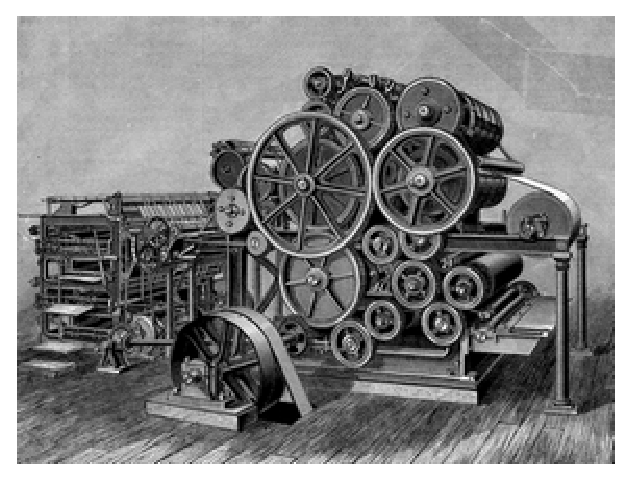
\includegraphics{knihtlac.eps}}
   			\caption{\textit{Prvý tlačiarenský lis}}
		\end{center}
	\end{figure}
	Ďalší výrazný posun v~tlači je zaznamenaný v 19. storočí prichodom nových technológií ako farebná tlač, \myuv{rotačka} a~ofsetová tlač.
\end{frame}

%~^~%~^~%~^~%~%~^~%~%~^~%~%~^~%~%~^~%~%~^~%~%~^~%~%~^~%~%~^~%~%~^~%

\begin{frame}{\emph{Pravidlá typografie}}
	Pre tvorbu typografických diel sa vyvinulo mnoho pravidiel, ku ktorým patria:
  \begin{itemize}
  \bigskip
		\item Optický stred
		\item Zlatý rez
		\item Normalizované formáty
    	\item \emph{\textbf{\color{red}Čitateľnosť}}
	\end{itemize} 
\begin{figure}
	\begin{center}
    	\scalebox{0.5}{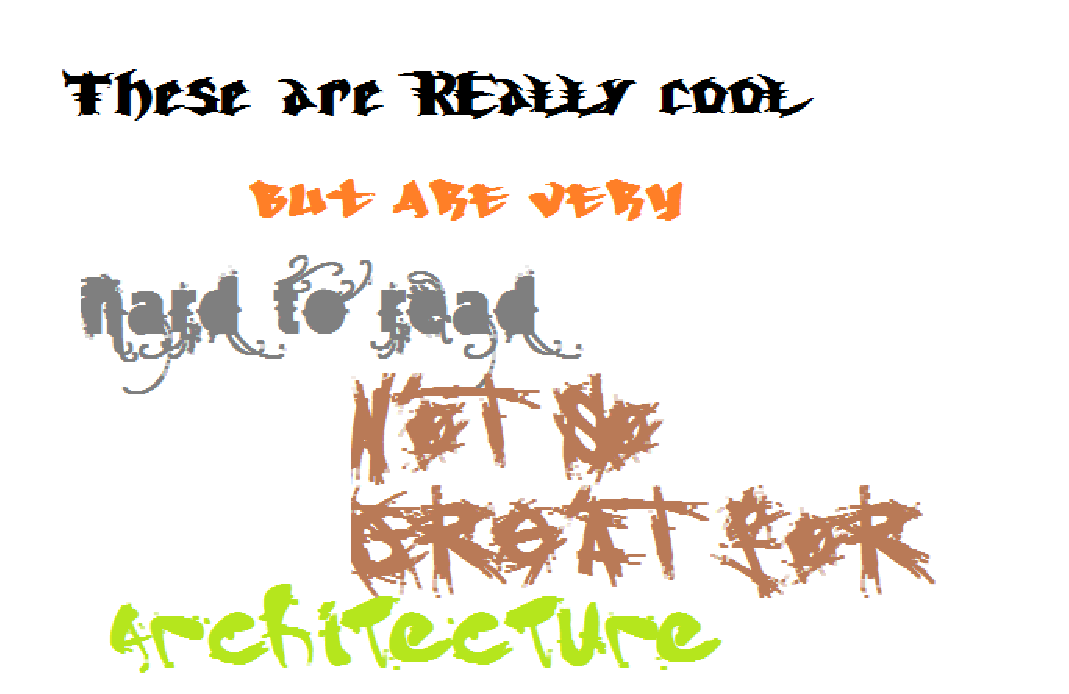
\includegraphics[width=0.8\textwidth]{unreadable.eps}}
    	\caption{Ukážka zlej čitateľnosti}
    \end{center}
\end{figure}
\end{frame}

%~^~%~^~%~^~%~%~^~%~%~^~%~%~^~%~%~^~%~%~^~%~%~^~%~%~^~%~%~^~%~%~^~%

\begin{frame}{\textsc{\large{Pravidlá typografie}}}
	Dobrá typografia totiž nie je vidieť, je nerušivým nástrojom k~odovzdaniu obsahu informácie.
	\bigskip
	\begin{figure}[ht]
		\begin{center}
			\scalebox{0.3}{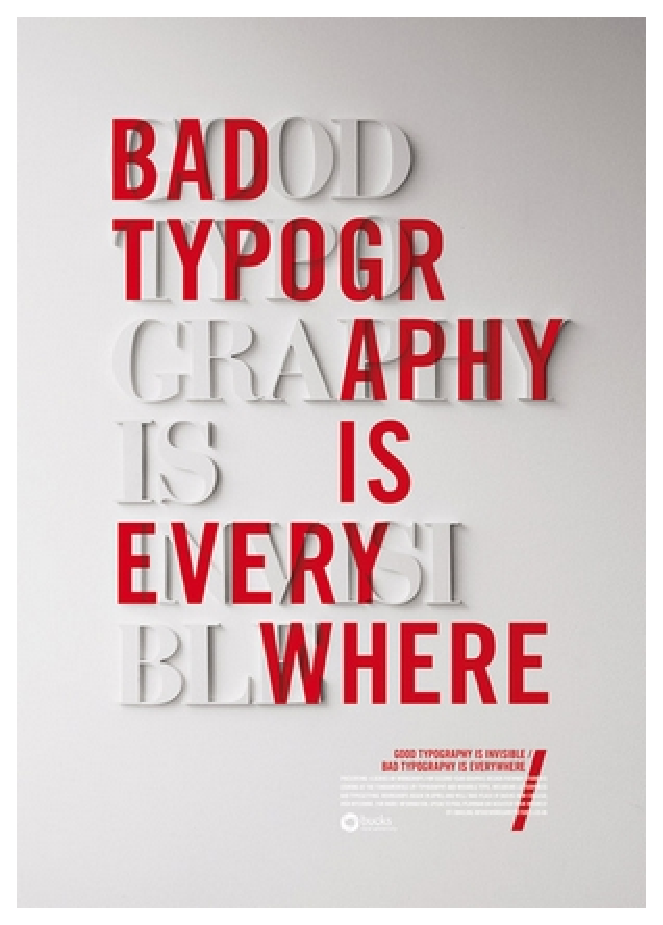
\includegraphics{typo2.eps}}
    		\caption{\textit{Ukážka ukážky \myuv{zlej} typografie}}
		\end{center}
	\end{figure}
\end{frame}

%~^~%~^~%~^~%~%~^~%~%~^~%~%~^~%~%~^~%~%~^~%~%~^~%~%~^~%~%~^~%~%~^~%

\begin{frame}{\textsc{\large{Pravidlá typografie}}}
	Základnou chybou sádzača\,--\,amatéra býva snaha dostať toho na stránku čo najviac bez ohľadu na čitateľnosť. Je dosť obtiažne vyjadriť správny postup vedúci k~optimálnej sadzbe kvantitatívne.
	\bigskip
	\begin{figure}[ht]
		\begin{center}
			\scalebox{0.7}{
\includegraphics{toosmall.eps}}
   			\caption{\textit{Ukážka dôsledku \myuv{nečitateľnosti}}}
		\end{center}
	\end{figure}
\end{frame}

%~^~%~^~%~^~%~%~^~%~%~^~%~%~^~%~%~^~%~%~^~%~%~^~%~%~^~%~%~^~%~%~^~%

\begin{frame}{\textsc{\large{\LaTeX}}}
	\begin{itemize}
		\item {\LaTeX} je vysoko kvalitný typografický systém určený pre profesionálne a~poloprofesionálne sádzanie dokumentov 
		\item Bol vyvinutý v roku 1985 Leslie Lamportom 
		\item Využíva ako formátovací jazyk sádzací systém {\TeX}
	\end{itemize}
	\begin{figure}[ht]
		\begin{center}
			\scalebox{0.8}{
\includegraphics{latex.eps}}
    		\caption{\textit{Ukážka zdrojového kódu v \LaTeX u}}
		\end{center}
	\end{figure}
\end{frame}

%~^~%~^~%~^~%~%~^~%~%~^~%~%~^~%~%~^~%~%~^~%~%~^~%~%~^~%~%~^~%~%~^~%

\begin{frame}{\emph{Koniec}}
	\vspace{\stretch{0.0075}}
	\centering
	\LARGE\textsc{Ďakujem za pozornosť\,\dots}
\end{frame}

%~^~%~^~%~^~%~%~^~%~%~^~%~%~^~%~%~^~%~%~^~%~%~^~%~%~^~%~%~^~%~%~^~%

\end{document}
